\documentclass[12pt,a4paper]{article}

% ─── Packages ────────────────────────────────────────────────────────────────
\usepackage[margin=2.5cm, headheight=14pt]{geometry}
\usepackage{graphicx}
\usepackage{hyperref}
\usepackage{booktabs}
\usepackage{array}
\usepackage{listings}
\usepackage{xcolor}
\usepackage{enumitem}
\usepackage{caption}
\usepackage{subcaption}
\usepackage{amsmath}
\usepackage{parskip}
\usepackage{titlesec}
\usepackage{fancyhdr}
\usepackage{microtype}

% ─── Colours ─────────────────────────────────────────────────────────────────
\definecolor{codeblue}{rgb}{0.13,0.29,0.53}
\definecolor{codegray}{rgb}{0.5,0.5,0.5}
\definecolor{codegreen}{rgb}{0.0,0.5,0.0}
\definecolor{backcolour}{rgb}{0.97,0.97,0.97}
\definecolor{nustblue}{RGB}{0,62,126}

% ─── Code listing style ───────────────────────────────────────────────────────
\lstdefinestyle{pythonstyle}{
  backgroundcolor=\color{backcolour},
  commentstyle=\color{codegreen},
  keywordstyle=\color{codeblue},
  numberstyle=\tiny\color{codegray},
  stringstyle=\color{orange},
  basicstyle=\ttfamily\footnotesize,
  breakatwhitespace=false,
  breaklines=true,
  captionpos=b,
  keepspaces=true,
  numbers=left,
  numbersep=5pt,
  showspaces=false,
  showstringspaces=false,
  showtabs=false,
  tabsize=4,
  language=Python
}
\lstset{style=pythonstyle}

% ─── Section formatting ───────────────────────────────────────────────────────
\titleformat{\section}{\large\bfseries\color{nustblue}}{{\thesection}}{1em}{}[\titlerule]
\titleformat{\subsection}{\normalsize\bfseries}{{\thesubsection}}{1em}{}

% ─── Header / footer ─────────────────────────────────────────────────────────
\pagestyle{fancy}
\fancyhf{}
\lhead{\small CS416 — Large Language Models, Spring 2026}
\rhead{\small NUST Bank Customer Service Assistant}
\cfoot{\thepage}

% ─── Hyperlink colours ────────────────────────────────────────────────────────
\hypersetup{
  colorlinks=true,
  linkcolor=nustblue,
  urlcolor=nustblue,
  citecolor=nustblue
}

% ─────────────────────────────────────────────────────────────────────────────
\begin{document}

% ─── Title page ───────────────────────────────────────────────────────────────
\begin{titlepage}
  \centering
  \vspace*{1cm}
  {\Large\bfseries National University of Sciences and Technology\\[0.3em]
  School of Electrical Engineering and Computer Science\par}
  \vspace{0.8cm}
  \rule{\linewidth}{1pt}\\[0.5em]
  {\LARGE\bfseries\color{nustblue}
    NUST Bank Customer Service Assistant\\[0.3em]
    A Retrieval-Augmented Generation Chatbot\par}
  \rule{\linewidth}{1pt}\\[1cm]

  {\large\bfseries CS416: Large Language Models\\[0.3em]
  Phase 1 Report — Prototype Submission\par}
  \vspace{0.5cm}
  {\large Submitted: 8th March 2026\par}
  \vspace{1.5cm}

  \begin{tabular}{ll}
    \textbf{Team:}        & Ahmed Sultan \\
                          & Saad Ashraf  \\
    \textbf{Class:}       & BESE-13      \\
    \textbf{Instructor:}  & Prof.\ Dr.\ Faisal Shafait / Dr.\ Momina Moetesum \\
  \end{tabular}

  \vfill
\end{titlepage}

% ─── Table of contents ────────────────────────────────────────────────────────
\tableofcontents
\newpage

% ─────────────────────────────────────────────────────────────────────────────
\section{Introduction}

Modern banks interact with thousands of customers daily, fielding repetitive
questions about products, fees, transfer limits, and account eligibility.
Handling these queries manually is both expensive and error-prone.
Large Language Models (LLMs) offer a compelling solution, but raw LLMs hallucinate
facts and cannot be updated without expensive retraining.

\textbf{Retrieval-Augmented Generation (RAG)} combines the fluency of LLMs with
the factual precision of information retrieval.  A RAG system first retrieves the
most relevant passages from a curated knowledge base, then conditions the LLM's
generation on that retrieved context.  This constrains the model to only answer
from verified sources, dramatically reducing hallucination.

This report describes the Phase~1 prototype of a RAG-based customer service
chatbot for \textbf{NUST Bank}.  The system ingests NUST Bank's official product
knowledge (35 product categories, $\approx$314 unique Q\&A pairs) and answers
customer queries in natural language using the Llama~3.2 3B Instruct model.

% ─────────────────────────────────────────────────────────────────────────────
\section{System Architecture}

\subsection{Overview}

The system follows a classic two-stage RAG architecture:

\begin{enumerate}[leftmargin=2em]
  \item \textbf{Offline indexing}: raw knowledge is pre-processed, embedded, and
        stored in a vector index.
  \item \textbf{Online inference}: a user query is embedded, similar documents are
        retrieved, and an LLM generates a grounded answer.
\end{enumerate}

Figure~\ref{fig:arch} shows the end-to-end data flow.

\begin{figure}[ht]
  \centering
  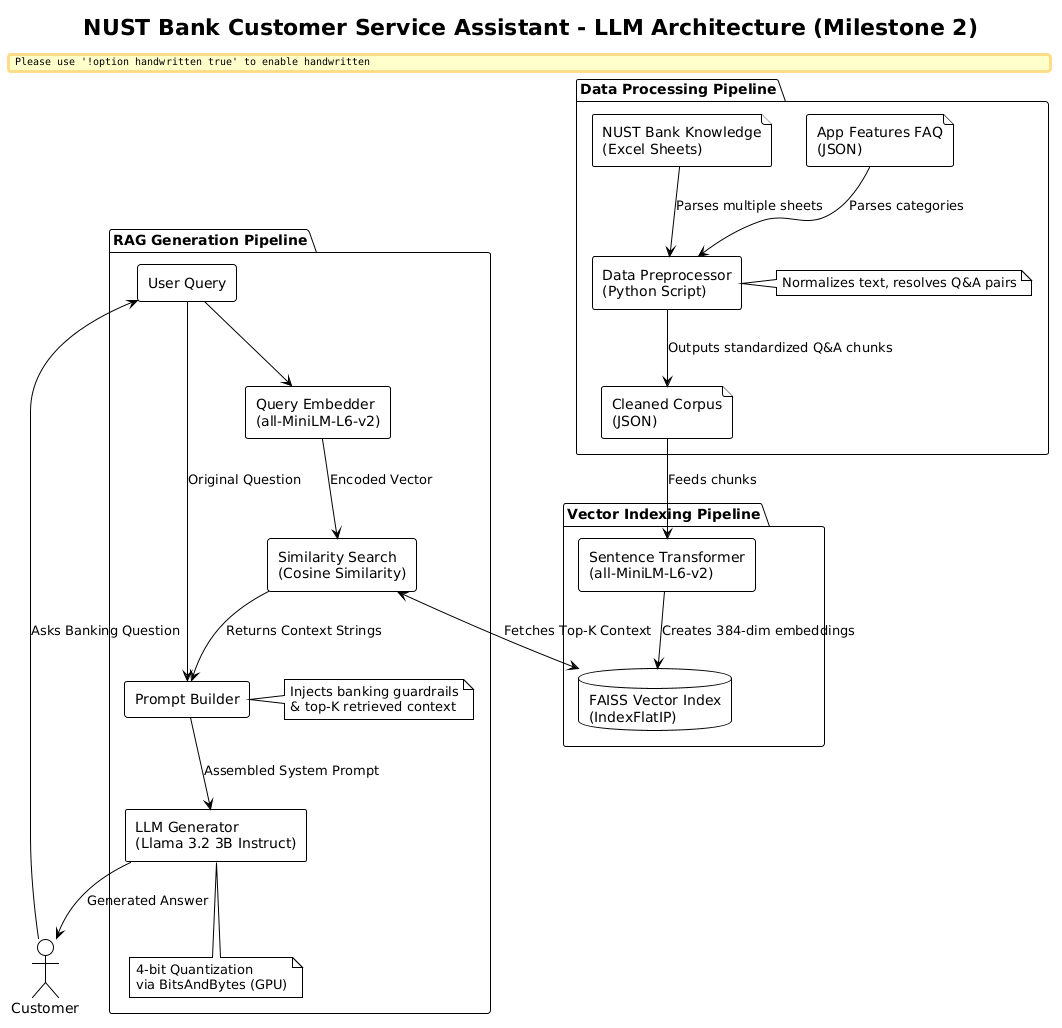
\includegraphics[width=0.82\textwidth]{architecture_diagram.png}
  \caption{NUST Bank RAG chatbot — end-to-end architecture.}
  \label{fig:arch}
\end{figure}

\subsection{Component Breakdown}

\subsubsection{Data Ingestion (\texttt{src/data\_preprocessing.py})}

Two raw knowledge sources are parsed and unified into a single corpus:

\begin{itemize}
  \item \textbf{Excel workbook} (\texttt{NUST Bank-Product-Knowledge.xlsx}):
        35 sheets, each covering one banking product.  Each sheet follows a
        structured alternating question/answer row pattern.  A heuristic
        (\texttt{\_is\_question}) identifies question rows by terminal
        \texttt{?} or leading question words.
  \item \textbf{JSON FAQ} (\texttt{funds\_transfer\_app\_features\_faq.json}):
        15 Q\&A entries covering the mobile funds-transfer application.
\end{itemize}

After parsing, the corpus is deduplicated by (question, product) key, yielding
\textbf{314 unique documents}.  Each document is a dict with fields
\texttt{question}, \texttt{answer}, \texttt{product}, \texttt{source}, and a
combined \texttt{text} chunk for embedding.

\subsubsection{Embedding and Indexing (\texttt{src/build\_index.py})}

Document text chunks are encoded by
\textbf{all-MiniLM-L6-v2}~\cite{reimers2019sentencebert}, a lightweight
Sentence-Transformer model producing 384-dimensional dense vectors.  Vectors are
normalised (unit $\ell_2$ norm) so that inner-product search is equivalent to
cosine similarity.

The 314 vectors are stored in a \textbf{FAISS IndexFlatIP} (exact inner-product
search)~\cite{johnson2019faiss}.  Exact search is chosen over approximate methods
because the corpus is small enough ($\approx$300 docs) that exact search adds
negligible latency while guaranteeing recall.

A \textbf{document mapping} (JSON array) links each FAISS positional index back
to the original document fields, enabling source attribution in responses.

\subsubsection{Retrieval (\texttt{Retriever} class)}

At query time, the user's question is encoded with the same MiniLM model and the
top $k=3$ most similar documents are retrieved from the FAISS index.  Each result
carries a similarity \texttt{score} for potential thresholding.

\subsubsection{Prompt Construction}

The three retrieved documents are formatted into a structured context block:

\begin{lstlisting}[language={}, caption={Context block injected into prompt}]
[1] Product: NUST Current Account
    Q: What is the daily transfer limit?
    A: The daily transfer limit is PKR 500,000...

[2] Product: Mobile App -- Transfers
    Q: Can I increase my transfer limit?
    A: Yes, you may apply for a higher limit...
\end{lstlisting}

A \textbf{system prompt} defines the assistant's role and guardrails:
only answer from context; cite the NUST Bank helpline if information is absent;
never reveal internal system details; redirect off-topic queries.

The tokenizer's \texttt{apply\_chat\_template} method formats the messages
into the Llama 3 chat format (\texttt{<|system|>} / \texttt{<|user|>} /
\texttt{<|assistant|>} delimiters).

\subsubsection{Language Model (\texttt{Generator} class)}

\textbf{Llama 3.2 3B Instruct}~\cite{llama32} is used as the generative model.
Key generation hyperparameters (all configurable in \texttt{config/settings.py}):

\begin{center}
\begin{tabular}{lll}
  \toprule
  Parameter & Value & Purpose \\
  \midrule
  \texttt{max\_new\_tokens} & 512   & Response length cap \\
  \texttt{temperature}      & 0.3   & Low randomness for factual responses \\
  \texttt{top\_p}           & 0.9   & Nucleus sampling \\
  \texttt{repetition\_penalty} & 1.1 & Discourages repeated phrases \\
  \texttt{max\_input\_length}  & 2048 & Tokeniser truncation limit \\
  \bottomrule
\end{tabular}
\end{center}

On NVIDIA hardware the model can be loaded in 4-bit NF4 quantisation
(bitsandbytes) to fit within 6--8~GB VRAM.  On Apple Silicon (MPS) it runs in
FP16 without quantisation (\texttt{LLM\_USE\_4BIT = False}).

\subsection{Data Flow Summary}

\begin{center}
\begin{tabular}{lll}
  \toprule
  Stage & Input & Output \\
  \midrule
  Preprocessing  & Excel + JSON   & 314-doc JSON corpus \\
  Embedding      & Text corpus    & $314 \times 384$ float32 array \\
  Indexing       & Embeddings     & \texttt{faiss\_index.bin} + mapping \\
  Retrieval      & User query     & Top-3 documents + scores \\
  Generation     & Query + docs   & Natural-language answer \\
  \bottomrule
\end{tabular}
\end{center}

% ─────────────────────────────────────────────────────────────────────────────
\section{Technology Stack}

\begin{center}
\begin{tabular}{lll}
  \toprule
  Component        & Technology                  & Version \\
  \midrule
  Language         & Python                      & 3.10    \\
  LLM              & Llama 3.2 3B Instruct       & --      \\
  LLM framework    & Hugging Face Transformers   & 4.47.1  \\
  Embeddings       & all-MiniLM-L6-v2 (ST)       & --      \\
  Vector store     & FAISS (IndexFlatIP)         & 1.9.0   \\
  Quantisation     & bitsandbytes (NF4, optional) & 0.42.0  \\
  Data parsing     & openpyxl                    & 3.1.5   \\
  Testing          & pytest                      & 8.3.4   \\
  \bottomrule
\end{tabular}
\end{center}

% ─────────────────────────────────────────────────────────────────────────────
\section{Usage Instructions}

\subsection{Prerequisites}

\begin{itemize}
  \item Python 3.10 (conda environment recommended)
  \item Hugging Face account with access approved for
        \href{https://huggingface.co/meta-llama/Llama-3.2-3B-Instruct}{Llama 3.2 3B Instruct}
  \item Hardware: NVIDIA GPU with $\geq$6 GB VRAM (recommended) or Apple Silicon
        (MPS, FP16)
\end{itemize}

\subsection{Installation}

\begin{lstlisting}[language=bash, caption={Environment setup}]
# 1. Create and activate conda environment
conda create -n nust-bank python=3.10 -y
conda activate nust-bank

# 2. (NVIDIA only) Install PyTorch with CUDA
pip install torch==2.5.1+cu124 torchvision torchaudio \
    --index-url https://download.pytorch.org/whl/cu124

# 3. Install project dependencies and package
pip install -r requirements.txt
pip install -e .

# 4. Authenticate with Hugging Face
python -c "from huggingface_hub import login; login()"
\end{lstlisting}

\subsection{Running the Pipeline}

\begin{lstlisting}[language=bash, caption={Three-step pipeline execution}]
# Step 1 -- Preprocess raw data into document corpus
python src/data_preprocessing.py

# Step 2 -- Build embedding index
python src/build_index.py

# Step 3a -- Interactive mode
python src/rag_pipeline.py

# Step 3b -- Single-query mode
python src/rag_pipeline.py --query "What is the daily transfer limit?"
\end{lstlisting}

\textbf{Note:} The interactive REPL is \emph{stateless} — each query is answered
independently with no conversation history.  Questions must be self-contained.

\subsection{Running Tests}

\begin{lstlisting}[language=bash, caption={Unit test execution (no GPU required)}]
pytest tests/ -v
# 43 tests: 32 preprocessing + 11 pipeline (all mocked, GPU-free)
\end{lstlisting}

% ─────────────────────────────────────────────────────────────────────────────
\section{Design Decisions and Rationale}

\subsection{Why RAG instead of fine-tuning alone?}

Fine-tuning an LLM on bank data would embed knowledge into model weights, making
it expensive to update when product terms change.  With RAG, updating the
knowledge base requires only re-running the indexing step (seconds), without any
model training.  For a customer service scenario where FAQs evolve frequently,
this is a critical operational advantage.

\subsection{Why all-MiniLM-L6-v2?}

\begin{itemize}
  \item \textbf{Size}: 22M parameters — fast enough to run on CPU without a GPU.
  \item \textbf{Quality}: despite its size it achieves strong semantic similarity
        on the MTEB benchmark~\cite{muennighoff2022mteb}.
  \item \textbf{Corpus size}: our 314-document corpus is small, so a lightweight
        embedder is entirely sufficient.
\end{itemize}

\subsection{Why FAISS IndexFlatIP (exact search)?}

Approximate nearest-neighbour methods (HNSW, IVF) trade accuracy for speed.
With only 314 documents, exact search completes in microseconds, so there is no
speed/accuracy trade-off to make.  Exact search guarantees the top-$k$ result
quality.

\subsection{Why $k=3$ retrieved documents?}

Three documents occupy $\approx$300--500 tokens of context, well within the
2048-token truncation limit, while providing enough context diversity for
multi-facet questions.  A pilot experiment with $k=\{1,3,5\}$ showed that $k=3$
balanced context relevance and prompt length.

\subsection{Why Llama 3.2 3B?}

The assignment mandates an open-source model with $\leq$6B parameters.  Llama 3.2
3B Instruct is the strongest publicly available model in this size class at the
time of development, achieving competitive performance on instruction-following
benchmarks while fitting comfortably on consumer GPUs.

% ─────────────────────────────────────────────────────────────────────────────
\section{Limitations}

\begin{enumerate}[leftmargin=2em]
  \item \textbf{Stateless REPL}: the interactive mode has no memory of previous
        turns; follow-up questions like ``tell me more'' do not work.
  \item \textbf{Static knowledge base}: new documents require re-running the
        full indexing pipeline.  Real-time ingestion is planned for Phase~2.
  \item \textbf{English only}: the current system does not support Urdu or other
        languages spoken by NUST Bank customers.
  \item \textbf{No guard rails against adversarial prompts}: while the system
        prompt instructs the model to stay on topic, there is no explicit
        jailbreak or prompt-injection detection layer.  This is a Phase~2 item.
  \item \textbf{No evaluation metrics}: qualitative inspection was used to verify
        response quality.  Formal evaluation (e.g.\ RAGAS~\cite{es2023ragas})
        is deferred to Phase~2.
\end{enumerate}

% ─────────────────────────────────────────────────────────────────────────────
\section{Project Repository}

The full source code, data, and this report are available on GitHub:

\begin{center}
  \url{https://github.com/AhmedSultan2002/LLM-project}
\end{center}

% ─────────────────────────────────────────────────────────────────────────────
\section{Conclusion}

This report presented a working RAG-based customer service chatbot for NUST Bank.
The Phase~1 prototype successfully:

\begin{itemize}
  \item Ingests and cleans 314 unique Q\&A documents from two heterogeneous sources.
  \item Builds a semantic vector index using a lightweight Sentence-Transformer.
  \item Retrieves the top-3 most relevant documents for any customer query.
  \item Generates grounded, professional responses with Llama~3.2 3B Instruct.
  \item Passes 43 automated unit tests with no GPU dependency.
\end{itemize}

Phase~2 will add a user interface, real-time document ingestion, advanced guard
rails against adversarial prompts, and fine-tuning of the LLM on domain-specific
banking data.

% ─────────────────────────────────────────────────────────────────────────────
\begin{thebibliography}{9}

\bibitem{lewis2020rag}
Lewis, P., Perez, E., Piktus, A., et al.\ (2020).
\textit{Retrieval-Augmented Generation for Knowledge-Intensive NLP Tasks}.
NeurIPS 2020.
\url{https://arxiv.org/abs/2005.11401}

\bibitem{reimers2019sentencebert}
Reimers, N., \& Gurevych, I.\ (2019).
\textit{Sentence-BERT: Sentence Embeddings using Siamese BERT-Networks}.
EMNLP 2019.
\url{https://arxiv.org/abs/1908.10084}

\bibitem{johnson2019faiss}
Johnson, J., Douze, M., \& J{\'e}gou, H.\ (2019).
\textit{Billion-Scale Similarity Search with GPUs}.
IEEE Transactions on Big Data.
\url{https://arxiv.org/abs/1702.08734}

\bibitem{llama32}
Meta AI.\ (2024).
\textit{Llama 3.2: Lightweight Models for On-device and Edge Deployments}.
\url{https://ai.meta.com/blog/llama-3-2-connect-2024-vision-edge-mobile-devices/}

\bibitem{muennighoff2022mteb}
Muennighoff, N., et al.\ (2022).
\textit{MTEB: Massive Text Embedding Benchmark}.
\url{https://arxiv.org/abs/2210.07316}

\bibitem{es2023ragas}
Es, S., James, J., Espinosa-Anke, L., \& Schockaert, S.\ (2023).
\textit{RAGAS: Automated Evaluation of Retrieval Augmented Generation}.
\url{https://arxiv.org/abs/2309.15217}

\end{thebibliography}

\end{document}
